% "summay.tex" %

\documentclass[12pt]{article}

\title{Simple Max-Cut on Unit Interval Graphs Findings Summary}
\author{Ethan Sifferman}
\date{December 2020}


\usepackage{changepage,amsmath,amssymb}

\usepackage{hyperref}

\usepackage{mathtools}
\DeclarePairedDelimiter{\floor}{\lfloor}{\rfloor}


\begin{document}
%%%%%%%%%%%%%%%%%%%%%%%%%%%%%%%%%%%%%%%%%%%%%%%%%%%%%%%%%%%%%%%%%%%%%%%%%%%%%%%%%%%%%%%%%%%%%%%%%%%%%%%%%%%%%%%%%%%%%%%%%

\setlength{\parindent}{0cm}
\setlength{\parskip}{1em}

\maketitle


%%%%%%%%%%%%%%%%%%%%%%%%%%%
%          Intro          %
%%%%%%%%%%%%%%%%%%%%%%%%%%%
\section{Introduction}


\subsection{Researchers}
\begin{itemize}
    \item Ethan Sifferman, ethanjsifferman@ucsb.edu
    \item Yuval Steinhart, yuval@ucsb.edu
    \item Ursula Hebert-Johnson, ursula@ucsb.edu
    \item Vaishali Surianarayanan, vaishali@ucsb.edu
    \item Daniel Lokshtanov, daniello@ucsb.edu
\end{itemize}

\subsection{Summary}
This paper is a summary of all the most important things we learned or discovered from May until December of 2020. We did not find an NP reduction nor an algorithm, but we expect that the problem is NP-Complete.

Note: This papers primarily covers what Ethan Sifferman worked on. Yuval Steinhart spent many hours on topics not even mentioned in this summary.

\subsection{Problem History}
In 1999, a polynomial time algorithm for Max-Cut on Unit Interval Graphs was proposed. We refer to this algorithm as the ``Every Other Algorithm".

In 2004, said algorithm was provided a counterexample, and a polynomial time algorithm on Split Unit Interval Graphs was found.

In 2017, a new Unit Interval Graph algorithm was proposed.

In Febuary 2020, said algorithm was disproved and replaced with a new, sub-exponential algorithm. We refer to this algorithm as the "Bubble Algorithm".

In May 2020, Unit Interval Graphs on Interval Graphs was found to be NP-Complete.

\subsection{Overview}
This is a list of all that we worked on.
\begin{itemize}
    \item Read the "Every Other Algorithm" paper and found the mistake.
    \item Simplified the problem into dealing with twin classes.
    \item Analyzed the problem using vector calculus.
    \item Discovered different edge cases for Unit Interval Graph structures.
    \item Designed an Algorithm Tester App.
    \item Proposed a (still unproven) algorithm to the path case. Referred to as the Sifferman Algorithm.
    \item Tried solving the Sifferman Algorithm base case with Wolfram.
    \item Proved the base case to the Sifferman Algorithm.
    \item Implimented the Sifferman Algorithm in a Web App.
    \item Read various papers related to Max-Cut on Unit Interval Graphs.
\end{itemize}




%%%%%%%%%%%%%%%%%%%%%%%%%%%
% Abstracting the Problem %
%%%%%%%%%%%%%%%%%%%%%%%%%%%
\section{Abstracting the Problem}
\subsection{Maximal Cliques and Twin Classes}
One of the first things we noticed about Interval Graphs is that they could be represented as a set of overlapping maximal cliques, ordered by endpoints.

\emph{``A graph $G$ is an interval graph iff and only if the maximal cliques of $G$ can be linearly ordered such that for each vertex $x$, the maximal cliques containing $x$ occur consecutively"} (Every Other Paper).

Then, we noticed that the intersections of maximal cliques provided twin classes. In unit interval graphs, these twin classes are disjoint and are able to be linearly ordered.

We can now abstract Unit Interval Graphs down into two integer arrays: $S$ and $C$ each with size $k$ such that \\
\underline{$k$ gives the number of twin classes}, \\
\underline{$S_i$ gives the size of the $i$th twin class}, and \\
\underline{$C_i$ gives the number of maximal cliques that contain the $i$th twin class}.

We can then abstract Max-Cut on Unit Interval Graphs into another integer array: $N$ such that \\
\underline{$N_i$ gives the number of verticies in twin class $i$ in partition $A$} and \\
\underline{$\bar{N_i}=(S_i - N_i)$ gives the number of verticies in twin class $i$ in partition $\bar{A}$}. \\
Note that $0 \leq N_i \leq S_i$.

Our new problem is: \\
Given $S$ and $C$, find $N$ such that $CUT(N_1, N_2, \ldots, N_k)$ is maximized.


\pagebreak

\subsection{Local Maximums}

A local maximum is defined as a cut arrangement $N$ such that either incrementing or decrementing any $N_i$ would result in the same or a lower $CUT$ value.

Each optimal $N_i$ must lie on either a boundary, ($0$ or $S_i$), or a local maximum. Given an arrangment $N$, we can always increase or match $CUT$ by applying a $Maximize$ operator to the $i$th twin class such that $N_i$ is set to $clamp(0, [local max], S_i)$\footnote{
    The $clamp(low, target, high)$ function will return
    $low$ if $target < low$,
    $high$ if $target > high$, and
    $target$ otherwise.
}. This operator is implemented in the Path Case Implimentation Website.

One of the biggest problems we ran into when writing proofs, was recognizing local maximums that were not global maximums. For example, a trivial local maximum would be $N := \left(\frac{S_1}{2}, \frac{S_s}{2}, \ldots, \frac{S_k}{2} \right)$. It is a local maximum because the cuts of all maximal cliques and twin classes are maximized. However, this $N$ is the same arrangment that the Every Other Algorithm chooses, which has trival counterexamples.




%%%%%%%%%%%%%%%%%%%%%%%%%%%
%      Notable Cases      %
%%%%%%%%%%%%%%%%%%%%%%%%%%%
\section{Notable Cases}
Our hope in finding edge cases was to find an algorithm that works for all Unit Interval Graphs. We also wanted to find the $CUT(N)$ formula in terms of $C$.

There are two cases for Unit Interval Graphs that we discussed: the Staircase Structure and the Path Structure. We have provided $C$ and $CUT(N)$ for both.

\pagebreak


\subsection{Staircase Structure}
A Staircase is a Unit Interval Graph with an odd number of twin classes, such that the middle twin class is contained in all maximal cliques.

$$C_{Staircase} = (1, 2, 3 \ldots p \ldots 3, 2, 1)$$

We could not find any algorithm for Staircases. Even by looking at many brute force solutions, there seemed to be \underline{no pattern} in optimal cuts. After a lot of work, we suspect that that Max-Cut on Staircase Unit Interval Graphs is NP-Complete.

\paragraph{$CUT(N)$ Formula} \leavevmode

\begin{itemize}
    \item $k :=$ \# of maximal cliques
    \item $p := \frac{k+1}{2} = $ \# of twin classes in each maximal clique
    \item $i :=$ the $i$th twin class
    \item $N_i :=$ size of $(i$th twin class $\cap A)$
\end{itemize}
\begin{align}
    CUT(N) &:= \sum_{i=1}^{k} \left[ \sum_{j=i}^{min((i+p-1), k)} \left[ N_i(S_j - N_j) + (s_i - n_i)n_j \right] - n_i (s_i - n_j) \right] \nonumber \\
    \nonumber \\
    \frac{\partial CUT}{\partial N_i} &:= \sum_{ j=max( 1, i-(p-1) ) }^{ min( i+(p-1), k ) } \left[ s_j - 2N_j \right] \nonumber
\end{align}


\pagebreak


\subsection{Path Structure}
A Path is a Unit Interval Graph with such that all maximal cliques have exactly two twin classes.

$$C_{Path} = (1, 2, 2 \ldots 2, 2, 1)$$

We believe that we have found a $O(n)$ algorithm. However, we have yet to prove it. Since we did not officially give it a name, while writing this summary, I have decided to name it the Sifferman Algorithm. If someone thinks of a better name for it though, I will happily let it be changed. :)

\paragraph{$CUT(N)$ Formula} \leavevmode
    
\begin{itemize}
    \item $k :=$ \# of maximal cliques
    \item $i :=$ the $i$th twin class
    \item $N_i :=$ size of $(i$th twin class $\cap~A)$
\end{itemize}
$$CUT(N) := \sum_{i=1}^{k} \left[ N_i(S_i - N_i) \right] + \sum_{i=1}^{k-1} \left[ N_i(S_{i+1} - N_{i+1}) + N_{i+1}(S_i - N_i) \right] \nonumber$$


\pagebreak


\paragraph{Sifferman Algorithm} \leavevmode

\fbox{\begin{minipage}{30em}

Let $n$ be a $\mathbb{R}$ array such that $|n| = k$.

$$\forall i : n_i := min \left( S_i, \frac{S_{i-1}+S_i+S_{i+1}}{2} \right)$$

\emph{Note: If $n_x$ or $S_x$ does not exist, use $0$.}

\[ 
    N_i =
    \begin{cases}
        n_i                     & i \in even \\
        \bar{n_i} = S_i - n_i   & i \in odd
    \end{cases}
\]

For all $i$, if $n_i$ or $\bar{n_i}$ is a non-integer, you may round either up or down.

\end{minipage}}

\begin{align}
    CUT(N) :=   & \sum_{i=1}^{k} \left[ \floor{n_i} (S_i - \floor{n_i}) \right] \nonumber \\
                & + \sum_{i=1}^{k-1} \left[ \floor{n_i}\floor{n_{i+1}} + (S_i - \floor{n_i})(S_{i+1} - \floor{n_{i+1}}) \right] \nonumber
\end{align}



\paragraph{Sifferman Algorithm $k=3$ Base Case}
Here, we prove that the Sifferman Algorithm works for when $k=3$ and $S_2 \geq S_1 \geq S_3$.

The Sifferman Algorithm sets $\bar{n_1}=\bar{n_3}=0$.

$CUT(N_{Sifferman}) = (S_1 + \floor{\bar{n_2}} + S_3)( S_2 - \floor{\bar{n_2}})$

Local max at
$$\bar{n_2} = \frac{ S_2 - ( S_1 + S_3) }{2}$$

We can prove $CUT(N_{Sifferman}) \geq CUT(N^*)$ by splitting the problem into two cases.


\underline{Case 1} $S_1 + S_3 \leq S_2$
\begin{align}
    &\therefore \bar{n_2} = \frac{ S_2 - ( S_1 + S_3) }{2} \nonumber \\
    &\therefore CUT(N_{Sifferman})_1 = \left( \frac{S_1 + S_2 + S_3}{2} \right)^2 \nonumber
\end{align}

$CUT(N_{Sifferman})_1$ cuts as many edges as an optimal cut on a clique. Therefore, $CUT(N_{Sifferman})_1 \geq CUT(N^*)_1$.

\underline{Case 2} $S_1 + S_3 \geq S_2$
\begin{align}
    &\therefore \bar{n_2} = 0 \nonumber \\
    &\therefore CUT(N_{Sifferman})_2 = (S_1 + S_3)S_2 \nonumber
\end{align}

We assume a counterexample $G$ such that $\bar{n_1}^* \neq 0$ and instead exists at a local maximum.

Local maximums at
\begin{align}
    \bar{n_1}^* &= \frac{2\bar{n_2}^* - S_1 + S_2}{2}                           \nonumber \\
    \bar{n_2}^* &= \frac{ 2\bar{n_{1}}^* - S_{1} + S_2 + 2\bar{n_{3}}^* - S_{3} }{2}
                                                                            \nonumber \\
                                                                            \nonumber \\
        &\therefore \bar{n_3}^* = \frac{S_3}{2}                               \nonumber \\
                                                                            \nonumber \\
    \therefore CUT(N^*)_2 &= \bar{n_1}^*(S_1-\bar{n_1}^*)
        + \left(\frac{2\bar{n_1}^* - S_1 + S_2}{2}\right)\left(\frac{S_1 - 2\bar{n_1}^* + S_2}{2}\right)
        + \frac{S_3^2}{4}                                                   \nonumber \\
        &+ \bar{n_1}^*\left(\frac{2\bar{n_1}^* - S_1 + S_2}{2}\right)
        + \frac{S_3}{2}\left(\frac{2\bar{n_1}^* - S_1 + S_2}{2}\right)        \nonumber \\
        &+ (S_1 - \bar{n_1}^*)\left(\frac{S_1 - 2\bar{n_1}^* + S_2}{2}\right)
        + \frac{S_3}{2}\left(\frac{S_1 - 2\bar{n_1}^* + S_2}{2}\right)        \nonumber \\
    \frac{dCUT(N^*)_2}{d\bar{n_1}^*} &\equiv 0                                        \nonumber
\end{align}

Since $\bar{n_1}^*$ does not change $CUT(N^*)_2$, $N^*$ could have $\bar{n_1}^* := \frac{S_2}{2}$.

$$\therefore CUT(N^*)_2 = \left(\frac{S_1}{2}\right)^2 + \left(\frac{S_2}{2}\right)^2 + \left(\frac{S_3}{2}\right)^2 + \frac{(S_1 + S_3)S_2}{2}$$



Now we can show that $CUT(N_{Sifferman})_2 \geq CUT(N^*)_2$.

Show
\begin{align}
    (S_1 + S_3)S_2  &\geq \left(\frac{S_1}{2}\right)^2 + \left(\frac{S_2}{2}\right)^2 + \left(\frac{S_3}{2}\right)^2 + \frac{(S_1 + S_3)S_2}{2} \nonumber \\
\nonumber \\
    2(S_1 + S_3)S_2 &\geq S_1^2 + S_2^2 + S_3^2     \nonumber \\
                    &\geq S_1S_2 + S_2^2 + S_3S_2   \nonumber \\
                    &\geq S_2^2 + (S_1 + S_3)S_2    \nonumber \\
                    &\geq 2(S_1 + S_3)S_2           \nonumber \\
                    &\checkmark                     \nonumber
\end{align}

The Sifferman Algorithm gives a cut no worse than optimal for both Case 1 and Case 2. Therefore, the Sifferman Algorithm produces optimal result for $k=3$ and $S_2 \geq S_1 \geq S_3$.




\paragraph{Sifferman Algorithm Equivalents} \leavevmode

\underline{Original Algorithm}

Recall, the Sifferman Algorithm does
$$\forall i : n_i := min \left( S_i, \frac{S_{i-1}+S_i+S_{i+1}}{2} \right)$$

\pagebreak


\underline{\emph{Start From Boundary} Variant}

A logically equivalent algorithm is to do

\fbox{\begin{minipage}{30em}

$$\forall i : n_i := S_i$$
Then apply the $Maximize$ operator on all $n_i$ in any order.

\end{minipage}}

This algorithm is equilavent because the Sifferman Algorithm will set all $n_i$ to their local maximum $L_i$ if $0 \leq L_i \leq S_i$, and $S_i$ otherwise.

Possibly this variant is easier to prove because each $n_i$ is as close as possible to their unbounded local maximums $n_i = \infty$.


\underline{\emph{Search for Largest} Variant}

The following is another logically equilavent algorithm:

\fbox{\begin{minipage}{30em}

For every $i$ with an unset $N_i$, iterate $i$ according to largest to smallest $S_i$. Set $N_{i-1}:=N_{i+1}:=0$ and $N_i := min \left( S_i, \floor{\frac{S_{i-1}+S_i+S_{i+1}}{2}} \right)$.

Then, if $N$ contains two consecutive $0$s or two consecutive $S_x$s, invert $N$ starting at the second of the consecutive elements such that all edges are cut between them.

\end{minipage}}

This algorithm is equivalent because both the Sifferman Algorithm and this variant will choose $N_i := \floor{\frac{S_{i-1}+S_i+S_{i+1}}{2}}$ only for twin classes with $S_i \geq S_{i-1}+S_{i+1}$. Also, both will alternate between $0$ and $S_i$ otherwise.

Possibly this variant is easier to prove because you can simply worry about triples, $N_{i-1}$, $N_{i}$, and $N_{i+1}$, one at a time.


\pagebreak


%%%%%%%%%%%%%%%%%%%%%%%%%%
%          Code          %
%%%%%%%%%%%%%%%%%%%%%%%%%%
\section{Code}

\begin{center}
    GitHub Repository   \\
    \url{https://github.com/E4tHam/MaxCut-UnitIntervalGraphs}
\end{center}

I spent nearly 100 hours working on implimentations of Max-Cut on Unit Interval Graphs. I learned a lot on how the structure can be built with code.



\subsection{Algorithm Tester}

\begin{center}
    GitHub Repository   \\
    \url{https://github.com/E4tHam/MaxCut-UnitIntervalGraphs/tree/main/algorithm-tester}
\end{center}

The purpose was to produce an app that allows for rapid testing of algorithm ideas.

\pagebreak


\paragraph{Features} \leavevmode

Has three Unit Interval Graph Types:
\begin{itemize}
    \item Random
    \item Path
    \item Staircase
\end{itemize}

Has three algorithms to use:
\begin{itemize}
    \item Brute Force Algorithm
    \item Every Other Approximation Algorithm
    \item Sifferman Algorithm on Path Graphs
\end{itemize}

Can cut according to file input.

Is easily expandable for more algorithms later.


\pagebreak


\subsection{Path Case Web App}

\begin{center}
    Web App             \\
    \url{https://maxcut.sifferman.dev/path/}
\end{center}
\begin{center}
    GitHub Repository   \\
    \url{https://github.com/E4tHam/MaxCut-UnitIntervalGraphs/tree/main/docs/path}
\end{center}


The purpose was to produce an app that allows for rapid testing of counterexamples and proofs for the Sifferman Algorithm on Path Graphs.



\paragraph{Explanation} \leavevmode

$S$ represents the size of each twin class.

Recall the Max-Cut problem separates a graph into two disjoint subsets, $A$ and $\bar{A}$. For the odd twin classes, the slider shows how many verticies are in subset $A$. For the even twin classes, the slider shows how many verticies are in subset $\bar{A}$.

A twin class $i$ with a picture [ / ] means that $n_i$ is locally maximal at $S_i$. A twin class $i$ with a picture [ \textbackslash ] means that $n_i$ is locally maximal at $0$. A twin class $i$ with a picture [ /\textbackslash ] means that $n_i$ is locally maximal between $0$ and $S_i$.

The [ Maximize ] button, applies the $Maximize$ operator, locally maximizing that twin class's $n$ value.



\pagebreak


\subsection{Base Case Solver}

\begin{center}
    GitHub Repository   \\
    \url{https://github.com/E4tHam/MaxCut-UnitIntervalGraphs/tree/main/wolfram}
\end{center}

I wrote this script to help solve the $k=3$ base case.


This script may not look like much, and it may not work, but it took MANY hours to learn Wolfram Language and try many things in order to try to prove the Sifferman Algorithm base case. My poblem was that the script would take way to long to complete. I spoke with a graduate student, Alex Meiburg, who has lots of Wolfram Language experience, and recieved this feedback:

\emph{
    It's unlikely there's a nice efficient solution to your problem, though. Even without the assumption that everything is an integer, this is \underline{linear-constrained} \\
    \underline{quadratic programming} which is in general going to be pretty hard. There are some cases where it's nice, like if the quadratic function is convex, but unfortunately this seems to not be convex. There are general algorithms for doing this symbolically, but they're sllooooow... I'll play with this some more tonight and get back to you, but unlikely there's a fast solution. :/
}

I ended up giving up after spening nearly 20 hours using different techniques to no success. Fortunetly, I ended up proving the $k=3$ case with algebra later.



\pagebreak


%%%%%%%%%%%%%%%%%%%%%%%%%%
%         Papers         %
%%%%%%%%%%%%%%%%%%%%%%%%%%

\section{Papers Read}
\emph{Sorry, I did not have time to get a real bibliography working. My LaTeX installation is a little wonky.}


\paragraph{SIMPLE MAX-CUT for unit interval graphs and graphs with few P4s} Hans L. Bodlaender, Ton Kloks, Rolf Niedermeier

Lemma 10 in this paper proposed the previously mentioned Every Other Algorithm. This paper was proven incorrect.

In the algebra portion of Lemma 10, we can see the term $a^2 - ad$, which subtracts all edges that would have been double-counted in the intersection of $G'$ and $C_t$. However, in the next step, they change $a^2 - ad$ to $-\frac{d^2}{4}$, which is less than the term in the previous step. Therefore, the error is that they forgot to switch the $\leq$ sign.

Interestingly, the Every-Other Algorithm seems to be quite a good approximation algorithm. There exists a trival proof to show it is a $\frac{1}{2}$-approximation. However, we suspect there exists a proof to show it is a $\frac{3}{4}$-approximation. However, we did not have time to come up with one.



\pagebreak


\paragraph{Unit Interval Graphs, Properties and Algorithms} Sayyed Bashir, Sadjad Hamid Zarrabi-Zadeh

The most important thing we discovered from this paper was Unit Interval Graph Forbidden Induced Subgraphs:
\begin{center}
    \makebox[\textwidth]{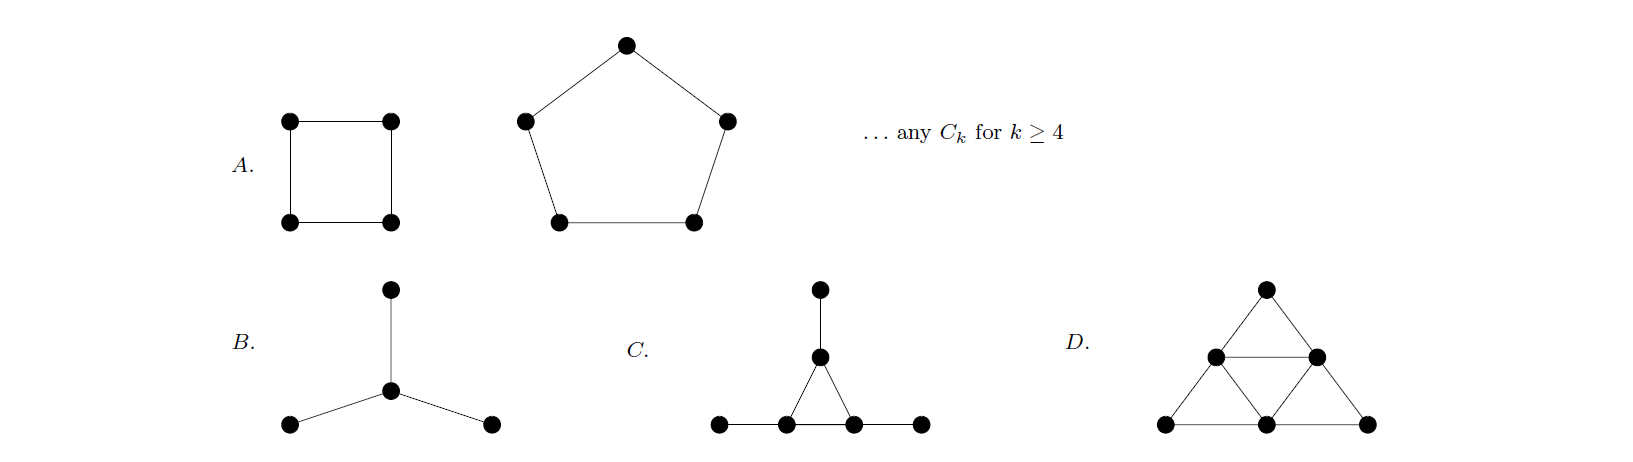
\includegraphics[width=\paperwidth]{forbidden.png}}
\end{center}

According to Figure 3 of this paper, \emph{A graph G is unit interval iff it does not contain any of these graphs as an induced
subgraph.}


\paragraph{Complexity of Maximum Cut on Interval Graphs} Ranendu Adhikary, Kaustav Bose, Satwik Mukherjee, Bodhayan Roy

In this paper, Max-Cut on Interval Graphs was found to be NP-Complete through a reduction from Max-Cut on Cubic Graphs to Max-Cut on Interval Graphs.

I lead a presentation discussing this paper for the UCSB Computer Science Theory weekly seminar on November 19th, 2020. Here is a link to the recording: \url{https://youtu.be/cUbd0lQF3SU}.



\pagebreak


\paragraph{$\mathcal{U}$-Bubble Model for Mixed Unit Interval Graphs and its
Applications: The MaxCut Problem Revisited} Jan Kratochvíl1, Tomáš Masarík, Jana Novotná

This paper proposes two parameterized algorithms and one sub-exponential algorithm utilizing a strategy called the bubble model.

The bubble model is a model for mixed unit interval graphs, which are unit interval graphs with either open or closed endpoints. The bubble model constructs a grid such that each vertex is placed in a cell, and a vertex can only have edges with cells in the same column. A mixed unit interval graph can be turned into a bubble model representation in $O(n)$ time.

Using a bubble model, there’s a sub-exponential $O( 2^{\sqrt{n}} )$ dynamic programming algorithm that computes the size of the max-cut.

For a bubble model with k columns, there is a $O( n^{k+5} )$ algorithm and for a model with k rows, there’s a $O( n^{4k+O(1)} )$ algorithm.

However, this paper is very complex and gave us a lot of difficulties while reading it. More time should be allocated towards reading this paper.



\section{Final Thoughts}

It has been a lot of fun diving into Max-Cut on Unit Interval Graphs. I now have a much better understanding of proofs, NP-Completeness, C++, reading research papers, approximation algorithms, and more.

Even though we may not have yet reached a solution, we learned a lot of important skills that we will carry through our acadmic years.



%%%%%%%%%%%%%%%%%%%%%%%%%%%%%%%%%%%%%%%%%%%%%%%%%%%%%%%%%%%%%%%%%%%%%%%%%%%%%%%%%%%%%%%%%%%%%%%%%%%%%%%%%%%%%%%%%%%%%%%%%
\end{document}
